\section{Мета роботи}
Набути навичок та закріпити знання при виконанні операцій
пошуку.

\section{Хід роботи}
  Розробити та налагодити програму, в якій реалізувати два алгоритми
пошуку відповідно до завдання. Порівняти алгоритми за часом роботи.\\

  На етапі тестування для кожного з алгоритмів (варіанти 4 – 15)
визначити кількість порівнянь у наборі даних з різною кількістю елементів
(20, 100, 1000, 10000) визначити час пошуку, заповнити таблицю за формою
табл. 9.1, побудувати графіки, зробити висновки. При роботі з текстом
(варіанти 1 – 3) змінювати довжину текста та зразка.\\

\textbf{Моє завдання:} Лінійний та лінійний з бар’єром пошуки у лінійному списку.\\

Для виконання лабораторної був використаний універсальний список з лабораторної 7.

\clearpage
\subsection{Реалізація функції лінійного пошуку}
\begin{lstlisting}[style=customc]
int linear_search_linked_list(Node *head, void *key, CompareFunc comparer)
{
  int comparisons = 0;
  Node *current = head;

  while (current)
  {
    comparisons++;
    if (comparer(current->data, key) == 0)
    {
      return comparisons;
    }
    current = current->next;
  }
  return comparisons;
}
\end{lstlisting}


\subsection{Реалізація функції лінійного пошуку з бар’єром}
\begin{lstlisting}[style=customc]
int linear_search_with_barrier(Node **head, void *key, CompareFunc comparer)
{
  if (!*head)
  {
    return 0;
  }

  insert_head_linked_list(head, key);
  int comparisons = 0;
  Node *current = *head;

  while (current)
  {
    comparisons++;
    if (comparer(current->data, key) == 0)
    {
      break;
    }
    current = current->next;
  }

  delete_node_linked_list(head, key, comparer, NULL);
  return comparisons;
}
\end{lstlisting}

\clearpage
\subsection{Реалізація додаткових методів для списку з цілими числами}
\begin{lstlisting}[style=customc]
int int_comparer(const void *a, const void *b)
{
  return *(int *)a - *(int *)b;
}

void fill_linked_list(Node **head, int size)
{
  for (int i = 0; i < size; i++)
  {
    int *value = (int *)malloc(sizeof(int));
    *value = generateRandomInt(1, 10000);
    insert_head_linked_list(head, value);
  }
}

void free_int_data(void *data)
{
  free(data);
}
\end{lstlisting}

\subsection{Реалізація лабораторної програми}
Було додано додаткову функцію для комфортного тестування та обробки результатів роботи функції.
\begin{lstlisting}[style=customc]
#include <stdio.h>
#include <stdlib.h>
#include <time.h>

#include "linked_list.h"
#include "general_utils.h"

void test_search(Node **head, void *key, CompareFunc comparer, int (*search_func)(Node *, void *, CompareFunc))
{
  clock_t start = clock();
  int comparisons = search_func(*head, key, comparer);
  clock_t end = clock();

  double time_taken_ms = ((double)(end - start)) / CLOCKS_PER_SEC * 1000;

  if (comparisons > 0 && comparisons <= 10000)
  {
    printf("Key found. Comparisons: %d \n\033[34m\033[0m Time: \033[32m%.3f\033[0m milliseconds\n", comparisons, time_taken_ms);
  }
  else
  {
    printf("Key not found. Comparisons: %d \n\033[34m\033[0m Time: \033[32m%.3f\033[0m milliseconds\n", comparisons, time_taken_ms);
  }
}

void task1()
{
  srand(time(NULL));

  int sizes[] = {20, 100, 1000, 10000};
  int num_sizes = sizeof(sizes) / sizeof(sizes[0]);

  for (int i = 0; i < num_sizes; i++)
  {
    int size = sizes[i];
    Node *head = NULL;

    printf("\n\033[34mTesting for list size: %d\033[0m\n", size);
    fill_linked_list(&head, size);

    int key = generateRandomInt(1, 1000);
    printf("Searching for key: %d\n\n", key);

    printf("\033[34m\033[0m Linear Search \033[34m\033[0m\n");
    test_search(&head, &key, int_comparer, linear_search_linked_list);
    puts("");
    printf("\033[34m\033[0m Linear Search with Barrier \033[34m\033[0m\n");
    test_search(&head, &key, int_comparer, (int (*)(Node *, void *, CompareFunc))linear_search_with_barrier);
    puts("\n------------------------------");

    destroy_linked_list(&head, free_int_data);
  }

  return 0;
}
\end{lstlisting}

\clearpage
\subsection{Результати роботи програми:}

\begin{figure}[h!]
    \centering
    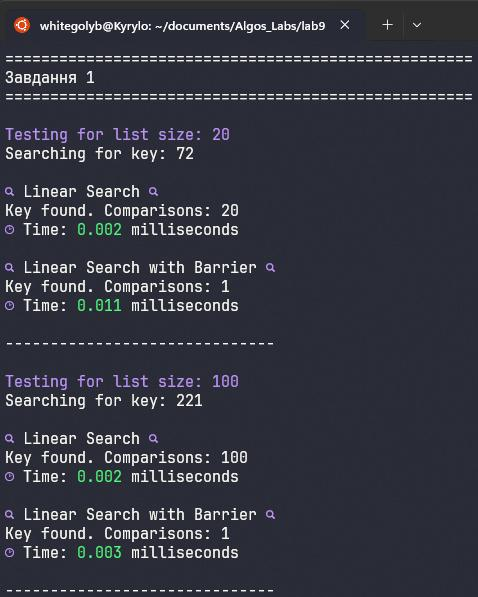
\includegraphics[width=15cm]{reports/algos/lab9/assets/1.jpeg}
    \caption{Результат пошуку для списку розміром 20 та 100}
\end{figure}

\begin{figure}[h!]
  \centering
  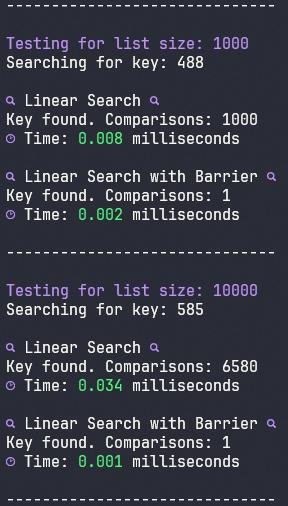
\includegraphics[width=13cm]{reports/algos/lab9/assets/2.jpeg}
  \caption{Результат пошуку для списку розміром 1000 та 10000}
\end{figure}


\clearpage
\begin{table}[htbp]
\caption{Таблиця результату для лінійного пошуку}
\begin{tabular}{|l|c|c|c|c|}
\hline
Кількість елементів & 20    & 100   & 1000  & 10000 \\ \hline
Кількість порівнянь & 1     & 100   & 1000  & 6580  \\ \hline
Час пошуку          & 0,002 & 0,002 & 0,008 & 0,034 \\ \hline
\end{tabular}
\end{table}

\vspace{-10pt} 


\begin{table}[htbp]
\caption{Таблиця результату для лінійного пошуку з бар’єром}
\begin{tabular}{|l|c|c|c|c|}
\hline
Кількість елементів & 20    & 100   & 1000  & 10000 \\ \hline
Кількість порівнянь & 1     & 1     & 1     & 1     \\ \hline
Час пошуку          & 0,011 & 0,003 & 0,002 & 0,001 \\ \hline
\end{tabular}
\end{table}

Графіки побудовані на основі таблиць
\begin{figure}[h!]
  \centering
  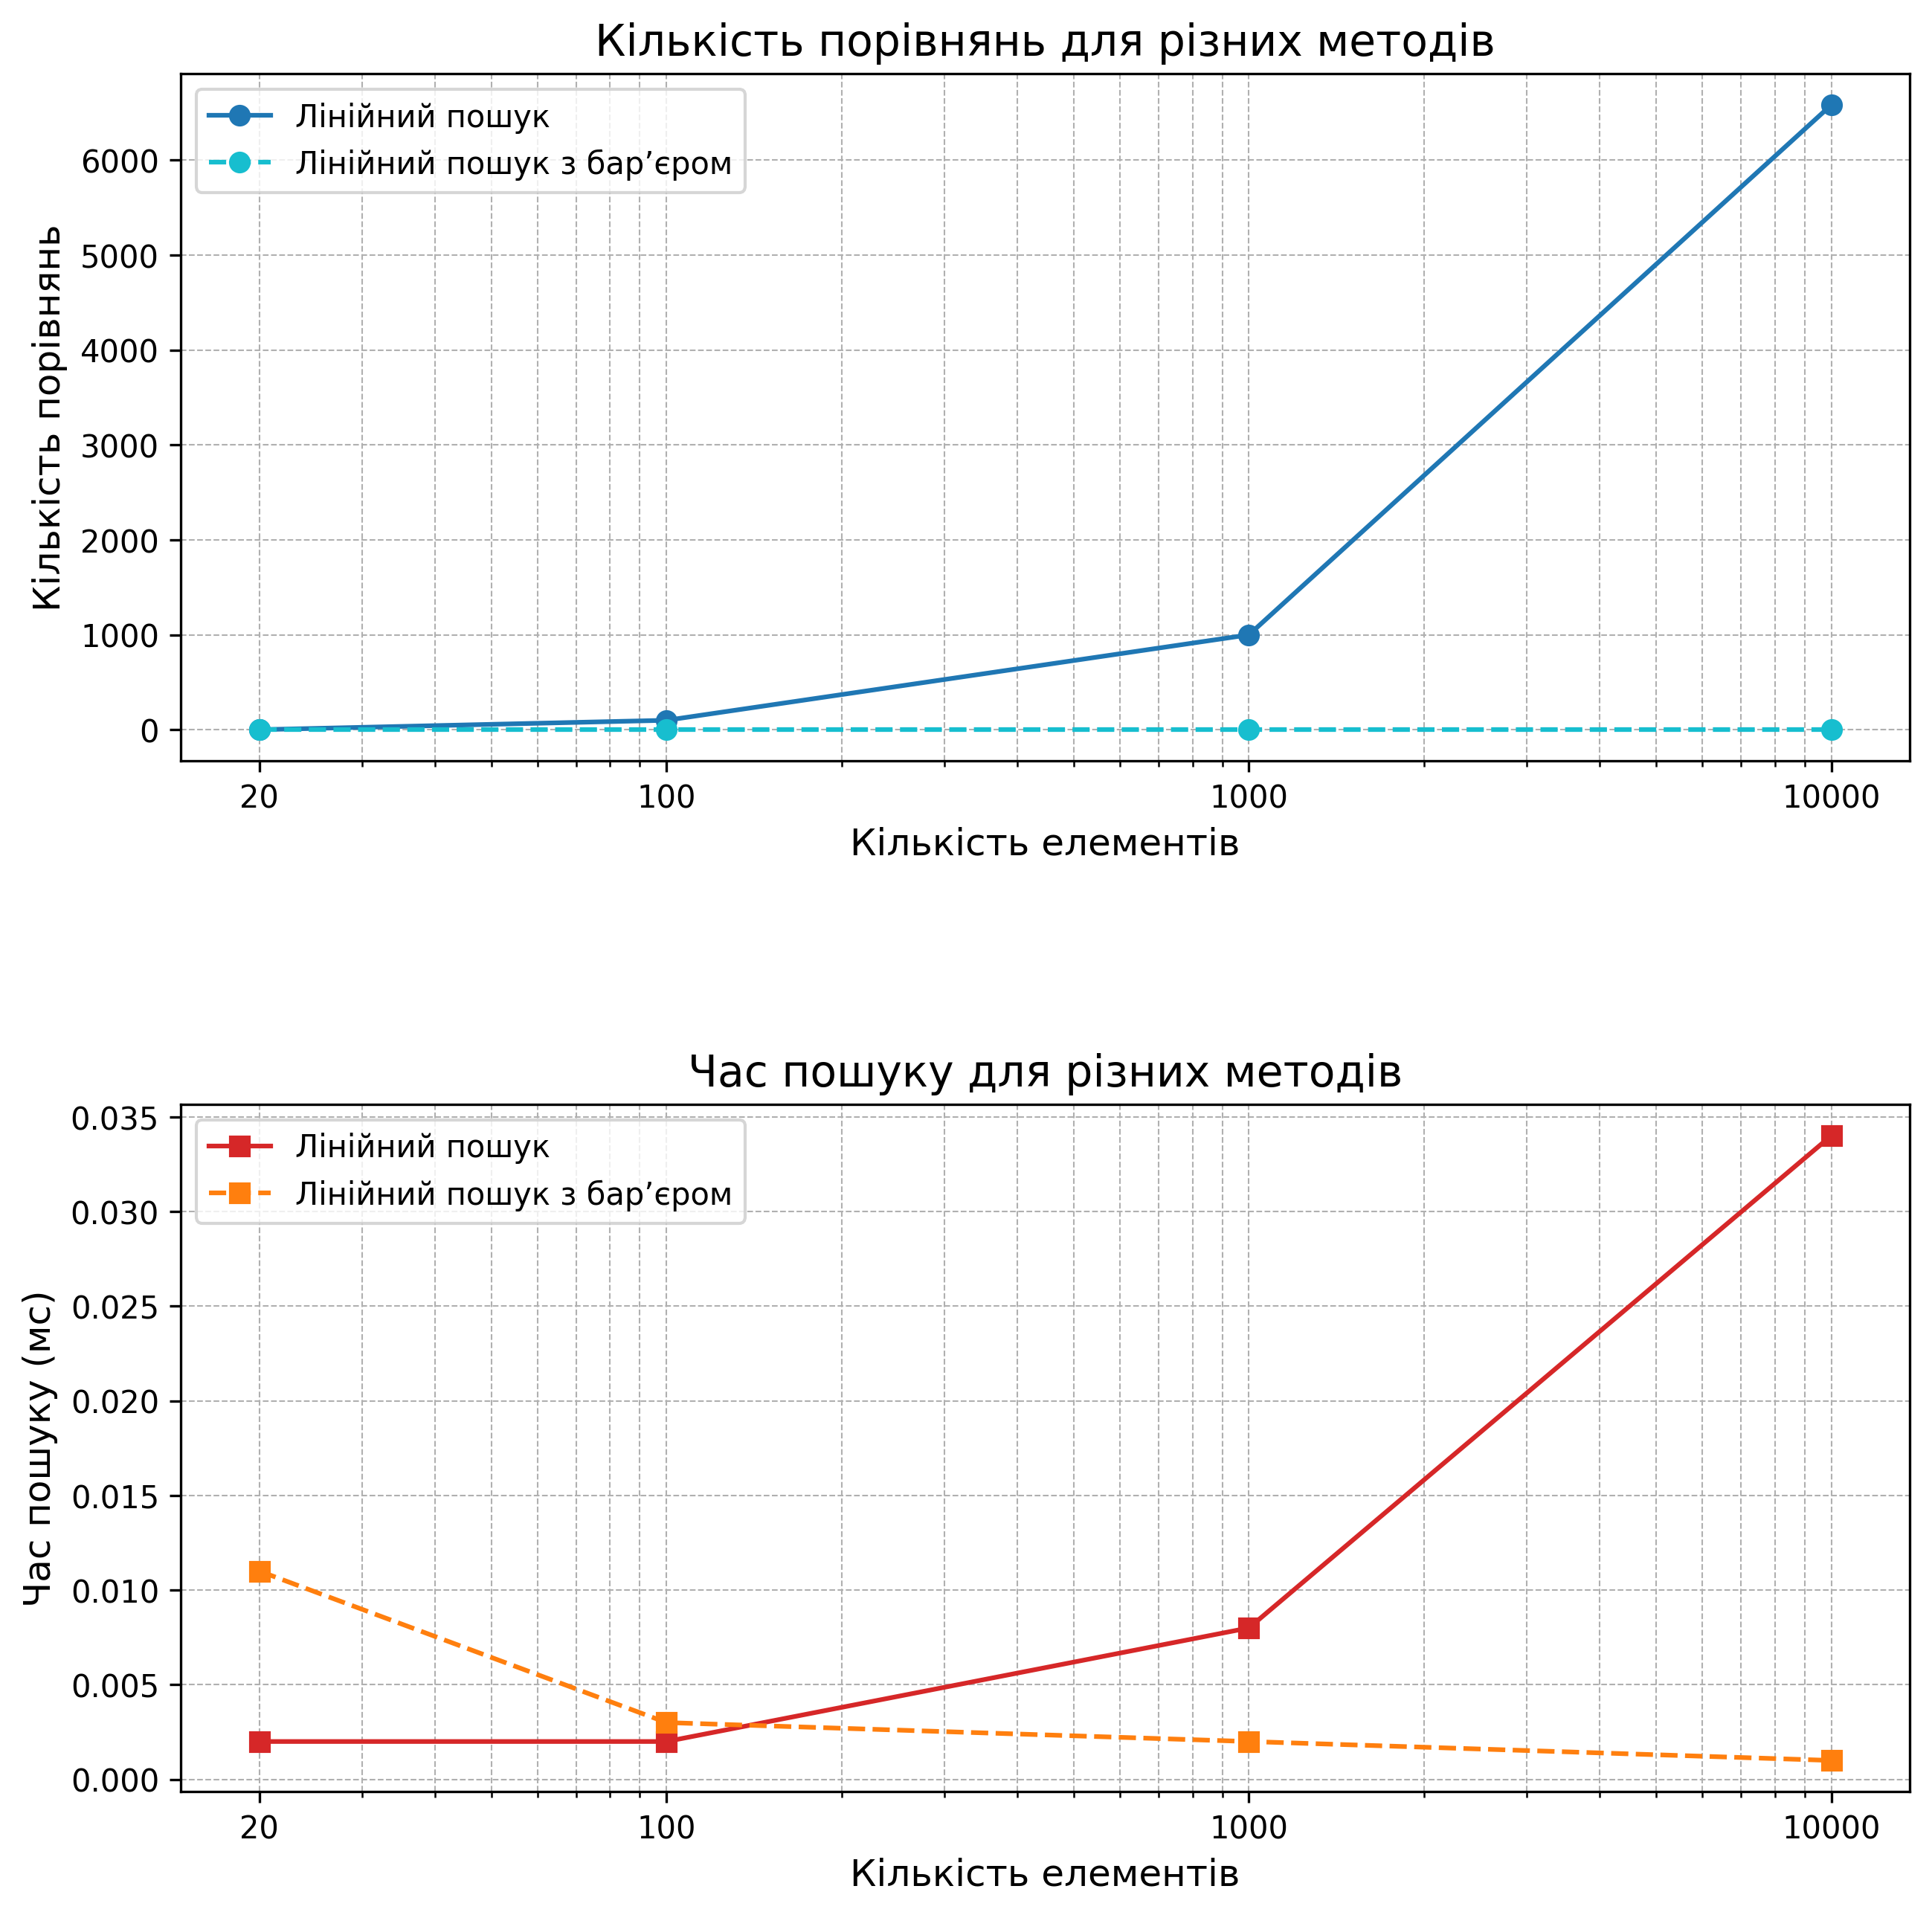
\includegraphics[width=17cm]{reports/algos/lab9/assets/plot.png}
\end{figure}



\clearpage
\section{Висновки}
В ході виконання лабораторної роботи було розроблено два методи пошуку ключа у лінійному списку та порівняно їх результати роботи. Порівняння представлено у вигляді таблиць та графіків за параметрами співпадінь та часу виконання відповідно. \\

Алгоритми лінійного пошуку краще за все підходять для списків, можна зазначити що пошук з бар’єром веде себе більш стабільніше за порівняннями при збільшенні обсягу списку та швидше за часом ніж лінійний.



